\documentclass[11pt,a4paper]{article}
\usepackage[utf8]{inputenc}
\usepackage[T1]{fontenc}
\usepackage[french]{babel}
\usepackage{lmodern}
\usepackage{amsmath,amssymb,bm}
\usepackage{geometry}
\geometry{margin=2.3cm}
\usepackage{graphicx}
\usepackage{booktabs,tabularx,array,longtable}
\usepackage{xcolor}
\usepackage[hidelinks]{hyperref}
\usepackage{caption}
\captionsetup{font=small,labelfont=bf}

\newcommand{\vect}[1]{\bm{#1}}
\newcommand{\hatv}[1]{\widehat{\bm{#1}}}
\newcommand{\Lam}{\bm{\Lambda}}
\newcommand{\Gam}{\bm{\Gamma}}
\newcommand{\Kv}{\mathbf{K}}
\newcommand{\code}[1]{\texttt{#1}}
\newcommand{\averif}{\textcolor{orange!80!black}{[à vérifier]}}

\title{Poutres géométriquement exactes (Simo--Reissner) dans fedoo\\[0.3em]
\large Théorie, implémentation, comparaison avec les approches corotationnelle\\
et de Kirchhoff, et intérêt des fibres en $\ln\mathbf V$ (corate \code{log\_R})}
\author{Note technique --- branche \code{feature/beam-simo-reissner}}
\date{19 octobre 2026}

\begin{document}
\maketitle

\begin{abstract}
Cette note décrit la poutre de Simo--Reissner (tige de Cosserat) ajoutée à fedoo
par l'option \code{BeamEquilibrium(kinematics="exact")}. Elle rappelle la
hiérarchie des modèles de tige (Kirchhoff, Reissner, Simo), situe l'approche
corotationnelle existante, détaille l'interpolation objective de
Crisfield--Jelenić, la linéarisation exacte et la symétrie de la tangente, puis
argumente le choix d'une loi de fibre écrite en déformation logarithmique avec la
contrainte de Kirchhoff, cohérente avec le corate \code{log\_R} de simcoon. Les
validations numériques (enroulement de Simo--Vu-Quoc, elastica de Reissner,
hélice, comparaison à un calcul 3D hyperélastique, toron de cinq brins avec
contact IPC) sont résumées. Les références marquées \averif{} ont été citées de
mémoire et doivent être contrôlées.
\end{abstract}

\tableofcontents

%======================================================================
\section{Notations et conventions}

\paragraph{Conventions.} Les vecteurs et tenseurs sont en gras, les scalaires en
italique ; un même symbole en gras et en italique désigne deux objets distincts
($\mathbf J$ jacobienne et $J$ constante de torsion, $\mathbf A$ tangente et $A$
aire). Pour $\mathbf v\in\mathbb R^3$, $\hatv v$ est la matrice antisymétrique
telle que $\hatv v\,\mathbf w=\mathbf v\times\mathbf w$. L'ordre des
déformations de poutre dans fedoo est
$[\Gamma_1,\Gamma_2,\Gamma_3,K_1,K_2,K_3]=[\varepsilon_x,\gamma_y,\gamma_z,\chi_x,\chi_y,\chi_z]$,
celui des efforts $[N,T_y,T_z,M_x,M_y,M_z]$. Le résidu est écrit en travail
virtuel interne positif et fedoo assemble $D=-R$ ; la matrice assemblée vaut
$+\partial R/\partial U$. Les inconnues \code{Rot} du Newton sont des
incréments de spin spatiaux : une triade nodale est mise à jour par
$\Lam\leftarrow\exp(\delta\hatv{\theta})\,\Lam$ et stockée dans
\code{sv["\_NodesRotationMatrix"]}.

\small
\begin{longtable}{>{\raggedright}p{3.1cm}p{11.9cm}}
\toprule
Symbole & Signification\\
\midrule
\endfirsthead
\toprule
Symbole & Signification\\
\midrule
\endhead
\multicolumn{2}{l}{\emph{Géométrie et cinématique de la tige}}\\
$S$ & abscisse curviligne de la ligne moyenne de référence ; $(\cdot)'=d(\cdot)/dS$\\
$y,\ z$ & coordonnées d'un point dans la section de référence\\
$\mathbf E_1,\mathbf E_2,\mathbf E_3$ & base orthonormée fixe ; $\mathbf E_1$ tangent à la ligne de référence (repère de référence de l'élément)\\
$\bm\varphi(S)$ & position courante de la ligne moyenne\\
$\mathbf x(S,y,z)$ & position courante d'un point matériel\\
$\Lam(S)\in SO(3)$ & triade (rotation) de la section ; $\Lam_i$ triade du nœud $i$\\
$\mathbf t_i=\Lam\mathbf E_i$ & directeurs de la section déformée ($\mathbf t_1$ normale à la section)\\
$\mathbf Q,\ \mathbf c$ & rotation et translation rigides superposées (tests d'objectivité)\\
\multicolumn{2}{l}{\emph{Déformations et efforts}}\\
$\Gam=(\Gamma_1,\Gamma_2,\Gamma_3)$ & déformations matérielles d'élongation ($\Gamma_1$) et de cisaillement ($\Gamma_2,\Gamma_3$)\\
$\Kv=(K_1,K_2,K_3)$ & courbures matérielles : torsion ($K_1$) et flexions ($K_2,K_3$)\\
$\bm\gamma=\Lam\Gam,\ \bm\kappa=\Lam\Kv$ & mêmes déformations en composantes spatiales\\
$\mathbf n,\ \mathbf m$ & résultantes matérielles d'effort et de moment, conjuguées de $\Gam$ et $\Kv$ ; $\mathbf s=(\mathbf n,\mathbf m)$\\
$N,\ T_y,\ T_z,\ M_x,\ M_y,\ M_z$ & composantes de $\mathbf n$ et $\mathbf m$ (effort normal, efforts tranchants, moments)\\
$W$ & densité linéique d'énergie de déformation de la section\\
$\delta_s,\ \delta_b$ & flèches de cisaillement et de flexion d'une console\\
\multicolumn{2}{l}{\emph{Section et matériau}}\\
$E,\ G,\ \nu$ & module d'Young, module de cisaillement $G=E/(2(1+\nu))$, coefficient de Poisson\\
$A,\ A_0$ & aire de la section (de référence)\\
$I_2,\ I_3$ ($I$) & moments quadratiques de flexion ; $J$ constante de torsion\\
$k$ & coefficient de correction de cisaillement ($k\approx0{,}886$ pour un cercle)\\
$r,\ L$ & rayon de la section et longueur de la tige (exemple de validation)\\
$\mathbf C_s$ & tangente de section $6\times6$, $\partial\mathbf s/\partial(\Gam,\Kv)$\\
\multicolumn{2}{l}{\emph{Rotations et outils de $SO(3)$}}\\
$\exp,\ \log$ & exponentielle et logarithme de $SO(3)$ (formule de Rodrigues)\\
$\mathbf p,\ x=|\mathbf p|$ & vecteur rotation quelconque et son angle\\
$\mathbf J(\mathbf p)$ & jacobienne gauche de $SO(3)$ : $\exp(\widehat{\mathbf p+\delta\mathbf p})=\exp(\widehat{\mathbf J\delta\mathbf p})\exp(\hatv p)$\\
$a,\ b,\ c$ ; $\alpha,\beta,\gamma$ & coefficients scalaires de $\mathbf J^{-1}$ et $\mathbf J$ ; leurs dérivées divisées par l'angle\\
$\bm\psi=\log(\Lam_1^T\Lam_2)$ & rotation relative de l'élément (repère du nœud 1)\\
$\Lam_r,\ \Lam_m$ & triade de référence de l'interpolation ; triade au point milieu\\
$\bm\psi^l_i$ & rotation locale du nœud $i$ relative à $\Lam_r$\\
$\delta\bm\theta_i$ & incrément de spin spatial du nœud $i$ (inconnue \code{Rot})\\
$\delta\bm\theta_m$ & spin du point milieu\\
$\mathbf T$ & matrice de transfert $\Lam_1\mathbf J(\bm\psi/2)\mathbf J^{-1}(\bm\psi)\Lam_1^T$ (interpolation CJ)\\
\multicolumn{2}{l}{\emph{Discrétisation et solveur}}\\
$L_0,\ L_e$ ($L$ dans les formules d'élément) & longueur de référence d'un élément\\
$\mathbf d$ & corde courante divisée par $L_0$ : $(\mathbf x_2-\mathbf x_1)/L_0$\\
$N_i(s)$ & fonctions de forme ; $s\in[0,L]$ abscisse dans l'élément\\
$\mathbf q,\ \delta\mathbf q$ & degrés de liberté nodaux de l'élément et leurs variations\\
$\mathbf B,\ \partial\mathbf B$ & $\partial(\Gam,\Kv)/\partial\mathbf q$ et ses dérivées directionnelles\\
$R,\ D,\ G_{\text{ext}}$ & résidu, vecteur assemblé par fedoo ($D=-R$), travail des charges extérieures\\
$\mathbf A$ & tangente assemblée $\partial R/\partial U$\\
$\mathbf G$ & raideur géométrique, $G_{ab}=\mathbf s\cdot\partial_b\mathbf B_{\cdot a}$\\
$\mathbf r_{\theta,n}$ & moment nodal interne assemblé au nœud $n$ (lignes \code{Rot} du résidu)\\
$\mathbf R_e,\ \bar{\mathbf q},\ \bar{\mathbf f},\ \bar{\mathbf K}$ & corotationnel : repère d'élément, ddl locaux, forces et raideur locales\\
$\ell,\ \ell_0$ & longueur courante et initiale de la corde (corotationnel)\\
$\alpha$ (solveur) & pas de la recherche linéaire\\
\multicolumn{2}{l}{\emph{Fibres en grandes déformations}}\\
$\mathbf g=(g_1,g_2,g_3)$ & déformation d'une fibre de section, $\mathbf g=\Gam+\Kv\times(0,y,z)^T$\\
$\lambda=1+g_1$ & élongation de la fibre ; $\ln\lambda$ sa déformation logarithmique\\
$\mathbf F$ & gradient de la transformation ; $\mathbf F=\mathbf R\mathbf U=\mathbf V\mathbf R$ décomposition polaire\\
$\mathbf R,\ \mathbf U,\ \mathbf V$ & rotation polaire, tenseurs d'élongation droit et gauche\\
$\ln\mathbf U,\ \ln\mathbf V$ & déformations logarithmiques (de Hencky) matérielle et spatiale\\
$\mathbf D,\ \mathbf D_e$ & taux de déformation eulérien et sa version tournée par le corate\\
$\mathbb A^R$ & opérateur du corate \code{log\_R} de simcoon ($\mathbf D_e=\mathbb A^R:\mathbf D$)\\
$\bm\sigma,\ \bm\tau=J_F\bm\sigma$ & contraintes de Cauchy et de Kirchhoff ($J_F=\det\mathbf F$)\\
$\mathbf P,\ \tilde{\mathbf P}=\Lam^T\mathbf P$ & premier Piola--Kirchhoff et sa version dans le repère de section\\
$\mathbf T_{\ln}$ & contrainte duale de $\ln\mathbf U$ ($\mathbf T_{\ln}=\mathbf R^T\bm\tau\mathbf R$ en coaxial)\\
$E_t$ & module tangent de fibre $d\tilde P_{11}/dg_1$\\
$\mathbf b=(1,0,0,0,z,-y)$ & vecteur reliant $g_1$ aux déformations de poutre\\
$\mathbf U_s$ & partie « cisaillement » $\mathbf I+\mathbf g\otimes\mathbf E_1$ (fibres \code{nshr=2})\\
$e$ & base du logarithme népérien ($e\approx2{,}718$)\\
$t$ & temps ; $\dot{(\ )}=d/dt$\\
\bottomrule
\end{longtable}
\normalsize

%======================================================================
\section{Hiérarchie cinématique des modèles de tige}

\subsection{La tige de Cosserat}
La position d'un point de la section s'écrit
\begin{equation}
\mathbf x(S,y,z)=\bm\varphi(S)+y\,\mathbf t_2+z\,\mathbf t_3,\qquad
\mathbf t_i=\Lam\,\mathbf E_i,
\end{equation}
où $S$ est l'abscisse curviligne de référence, $(y,z)$ les coordonnées dans
la section, $\bm\varphi$ la position de la ligne moyenne, $\Lam$ la rotation de la
section et $\mathbf t_i$ ses directeurs ($\mathbf E_i$ base fixe, $\mathbf E_1$
tangent à la ligne de référence). La configuration est donc
$(\bm\varphi,\Lam)\in\mathbb R^3\times SO(3)$. Les déformations
matérielles sont
\begin{equation}
\Gam=\Lam^T\bm\varphi'-\mathbf E_1,\qquad \hatv{K}=\Lam^T\Lam',
\end{equation}
et leurs homologues spatiaux $\bm\gamma=\Lam\Gam$, $\bm\kappa=\Lam\Kv$.
Sous un mouvement rigide superposé
$(\bm\varphi,\Lam)\mapsto(\mathbf Q\bm\varphi+\mathbf c,\mathbf Q\Lam)$,
$\Gam$ et $\Kv$ sont inchangés : ce sont des mesures objectives
\cite{reissner1981,simo1985}. Pour $\Lam\simeq\mathbf I+\hatv\theta$ on
retrouve la poutre de Timoshenko de fedoo : $\Gamma_2=v'-\theta_z$,
$\Gamma_3=w'+\theta_y$. Une section élastique ($E$ module d'Young, $G$ module de cisaillement, $A$
aire, $I_2,I_3$ moments quadratiques, $J$ constante de torsion, $k$ coefficient de
cisaillement) dérive du potentiel
\begin{equation}
W=\tfrac12\big(EA\,\Gamma_1^2+kGA(\Gamma_2^2+\Gamma_3^2)+GJ\,K_1^2+EI_2K_2^2+EI_3K_3^2\big).
\end{equation}

\subsection{Kirchhoff, Reissner, Simo}
\begin{center}
\small
\begin{tabularx}{\linewidth}{>{\raggedright}p{3.6cm}>{\raggedright}X>{\raggedright\arraybackslash}X}
\toprule
Modèle & Contrainte cinématique & Espace de configuration\\
\midrule
Kirchhoff (1859) \cite{kirchhoff1859}, Love \cite{love1927} &
$\Gamma_2=\Gamma_3=0$ (section normale à l'axe) ; inextensible si en plus $\Gamma_1=0$ &
ligne moyenne + torsion ; $\mathbf t_1=\bm\varphi'/\|\bm\varphi'\|$ ; exige une ligne $C^1$\\
Reissner 1972 (plan) \cite{reissner1972}, 1981 (3D) \cite{reissner1981} &
aucune : $\Gam$ et $\Kv$ indépendants & $\mathbb R^3\times SO(3)$\\
Simo 1985 \cite{simo1985}, Simo--Vu-Quoc 1986 \cite{simovuquoc1986} &
mêmes déformations & dynamique 3D, linéarisation cohérente sur $SO(3)$\\
\bottomrule
\end{tabularx}
\end{center}
Tous ces modèles négligent la déformation de la section dans son plan
(contraction de Poisson), le gauchissement et le couplage triaxial (la loi est une
loi en résultantes) \cite{antman2005}. Kirchhoff néglige en plus l'énergie de
cisaillement.

\subsection{Quand le cisaillement compte}
Pour une console de longueur $L$ et de rayon $r$ chargée en bout, le rapport des
flèches de cisaillement $\delta_s$ et de flexion $\delta_b$ vaut
\begin{equation}
\frac{\delta_s}{\delta_b}=\frac{3EI}{kGAL^2}
\;\overset{\text{cercle}}{=}\;\frac{3(1+\nu)}{2k}\Big(\frac rL\Big)^2\approx 2{,}2\Big(\frac rL\Big)^2
\quad(\nu=0{,}3,\ k\approx0{,}886).
\end{equation}
Pour une tige élancée ($L/r>50$) le cisaillement est négligeable globalement,
mais il gouverne une couche limite de quelques diamètres près des encastrements
et des charges concentrées, où la rotation de la section s'écarte de celle de la
tangente. C'est exactement ce que montre la comparaison au calcul 3D
(section~\ref{sec:valid}) : à $0{,}1L$ la section a tourné de $34^\circ$ en 3D
comme dans la tige, alors qu'un modèle de Kirchhoff imposerait l'angle de la
tangente. Pour des fils très élancés (rapport $>1000$), Meier, Popp et Wall
\cite{meier2019} montrent que les éléments de Kirchhoff sont plus efficaces : le
conditionnement des éléments de Reissner croît comme
$EA/(EI/L_e^2)\propto(L_e/r)^2$.

%======================================================================
\section{L'approche corotationnelle}

\subsection{Principe}
Dans l'approche corotationnelle \cite{belytschko1973,rankin1986,crisfield1990,nouromid1991,crisfield1997,battini2002,felippa2005},
un repère rigide $\mathbf R_e(\mathbf q)$ est attaché à chaque élément (corde et
triades nodales). Avec $\ell$ et $\ell_0$ les longueurs courante et initiale de la
corde, les degrés de liberté déformationnels locaux sont
$\bar{\mathbf q}=(\ell-\ell_0,\bar{\bm\theta}_1,\bar{\bm\theta}_2)$ avec
$\bar{\bm\theta}_i=\log(\mathbf R_e^T\Lam_i\Lam_{0i}^T\mathbf R_{e0})$, et une
poutre linéaire en petites déformations donne $\bar{\mathbf f}=\bar{\mathbf K}\bar{\mathbf q}$.
Dans une version cohérente, $\mathbf f=\mathbf B^T\bar{\mathbf f}$ avec
$\mathbf B=\partial\bar{\mathbf q}/\partial\mathbf q$ (rotation et projecteur),
$\mathbf q$ désignant les ddl globaux de l'élément :
la force est alors le gradient de $\tfrac12\bar{\mathbf q}^T\bar{\mathbf K}\bar{\mathbf q}$.

\subsection{Limites}
\begin{itemize}
\item La loi locale est en petites déformations : un allongement ou un
cisaillement fini sort du cadre, quel que soit le maillage. La rotation relative
dans l'élément, de l'ordre de $\tfrac12|K|L_e$, doit rester petite.
\item Le résultat dépend de la définition du repère d'élément (corde ou triade
moyenne, invariance à l'ordre des nœuds) \cite{felippa2005} \averif.
\item Dans fedoo, la force corotationnelle est la force locale tournée
historique, sans projecteur conjugué en énergie (docstring de
\code{\_beam\_tangent.py}) : elle ne dérive pas d'un potentiel et sa tangente
cohérente (\code{consistent\_tangent=True}) est non symétrique, même à
l'équilibre.
\item La formulation est en lagrangien réactualisé ; \code{nlgeom="TL"}
donnait silencieusement un résultat faux (cordes lues sur le maillage initial)
et lève désormais une erreur.
\end{itemize}

\subsection{Lien avec Simo--Reissner}
Pour une section élastique et de petites déformations, l'élément corotationnel
coïncide avec un élément de Reissner au premier ordre en rotation relative ;
l'écart est en $O((KL_e)^2)$ et les deux convergent vers la même solution
continue quand $h\to0$ \cite{crisfield1997,battini2002} \averif. La différence de
fond est donc constitutive et structurelle (loi locale linéaire, absence de
potentiel) plutôt que cinématique.

%======================================================================
\section{Interpolation des rotations : le schéma de Crisfield--Jelenić}

\subsection{Le problème d'objectivité}
Crisfield et Jelenić \cite{crisfield1999} ont montré que :
\begin{itemize}
\item interpoler additivement les rotations incrémentales spatiales, comme
Simo--Vu-Quoc \cite{simovuquoc1986}, avec la triade stockée aux points de Gauss,
rend les déformations dépendantes du chemin et non objectives ;
\item interpoler additivement les vecteurs rotation totaux
\cite{ibrahimbegovic1995,cardona1988} est indépendant du chemin mais non
objectif.
\end{itemize}
Le remède consiste à interpoler des rotations \emph{locales} relatives à une
triade de référence :
$\Lam(s)=\Lam_r\exp\big(\sum_iN_i\hatv\psi^l_i\big)$,
$\bm\psi^l_i=\log(\Lam_r^T\Lam_i)$ \cite{crisfield1999,jelenic1999}. Romero
\cite{romero2004} compare ces schémas : seuls les schémas en rotations relatives
et en directeurs \cite{romero2002,betsch2002} sont objectifs et indépendants du
chemin.

\subsection{Réduction à l'élément à deux nœuds}
Soit $\bm\psi=\log(\Lam_1^T\Lam_2)$ la rotation relative de l'élément, exprimée
dans la triade du nœud 1, et $\Lam_r=\Lam_1\exp(\hatv\psi/2)$. On a
$\bm\psi^l_1=-\bm\psi/2$ et $\bm\psi^l_2=\bm\psi/2$ ; ces vecteurs sont coaxiaux,
les exponentielles commutent et
\begin{equation}
\Lam(s)=\Lam_1\exp\!\Big(\frac sL\hatv\psi\Big)
\end{equation}
est la géodésique de $SO(3)$. Donc $\hatv K=\Lam^T\Lam'=\hatv\psi/L$ exactement
sur tout l'élément ($s\in[0,L]$ abscisse dans l'élément, $L=L_0$ sa longueur de
référence). Avec $\bm\varphi'=\mathbf d=(\mathbf x_2-\mathbf x_1)/L_0$ (corde
courante rapportée à la longueur de référence) et un point de Gauss au milieu,
où la triade vaut $\Lam_m$ :
\begin{equation}
\boxed{\;\Gam=\Lam_m^T\mathbf d-\mathbf E_1,\qquad \Lam_m=\Lam_1\exp(\hatv\psi/2),\qquad \Kv=\bm\psi/L\;}
\end{equation}
C'est exactement ce que calcule \code{\_kinematics\_3d}
(\code{fedoo/weakform/\_beam\_exact.py}), dans le repère de référence de
l'élément où les triades de référence valent l'identité. En 2D, $SO(2)$ est
commutatif et $\theta_m=\tfrac12(\theta_1+\theta_2)$ est exact et objectif.

\paragraph{Propriétés.}
\begin{itemize}
\item \emph{Objectivité} : sous $\Lam_i\to\mathbf Q\Lam_i$, $\mathbf x\to\mathbf Q\mathbf x$,
$\bm\psi$ est invariant, $\Lam_m\to\mathbf Q\Lam_m$, $\mathbf d\to\mathbf Q\mathbf d$.
\item \emph{Indépendance du chemin} : les déformations ne dépendent que de
l'état nodal courant ; une boucle fermée de rotations ne laisse aucune
déformation (testé).
\item \emph{Condition de maillage} : $|K|L_e<\pi$ (coupure du logarithme).
Les rotations nodales sont stockées comme matrices, sans singularité de vecteur
rotation total.
\item \emph{Un point de Gauss} : 12 ddl $-$ 6 modes rigides $=$ 6 modes de
déformation, et un point fournit 6 déformations indépendantes : rang exact,
pas de mode parasite. Le cisaillement constant par élément supprime le
verrouillage ; la quadrature au point milieu donne la convergence en $O(h^2)$
observée.
\end{itemize}

\subsection{Outils sur $SO(3)$}
Pour un vecteur rotation $\mathbf p$ d'angle $x=|\mathbf p|$, la jacobienne gauche
$\mathbf J$ relie une variation de $\mathbf p$ au spin produit,
$\exp(\widehat{\mathbf p+\delta\mathbf p})=\exp(\widehat{\mathbf J\delta\mathbf p})\exp(\hatv p)$ ;
elle et son inverse valent
\begin{equation}
\mathbf J(\mathbf p)=\mathbf I+\frac{1-\cos x}{x^2}\hatv p+\frac{x-\sin x}{x^3}\hatv p^{\,2},\qquad
\mathbf J^{-1}(\mathbf p)=\mathbf I-\tfrac12\hatv p+\frac1{x^2}\Big(1-\frac x2\cot\frac x2\Big)\hatv p^{\,2}.
\end{equation}
Sous raffinement, $\bm\psi=O(KL_e)\to0$ : la plupart des éléments sont dans le
régime des petits angles, où les formes fermées des dérivées des coefficients
(qui entrent dans $\partial\mathbf B$) subissent une annulation catastrophique
(8 chiffres perdus vers $0{,}05$~rad). Le module \code{fedoo/util/so3.py} utilise
des séries de Taylor à 10 termes jusqu'à 1~rad (rayon de convergence $2\pi$) ;
l'erreur reste sous $10^{-13}$ de part et d'autre du seuil (test contre
\code{mpmath}).

%======================================================================
\section{Forme faible, linéarisation, symétrie}

\subsection{Variations}
Pour des spins spatiaux $\Lam_i\leftarrow\exp(\delta\hatv\theta_i)\Lam_i$ :
\begin{align}
\delta\bm\psi&=\mathbf J^{-1}(\bm\psi)\,\Lam_1^T(\delta\bm\theta_2-\delta\bm\theta_1),\\
\delta\bm\theta_m&=\Big(\mathbf I-\tfrac12\mathbf T\Big)\delta\bm\theta_1+\tfrac12\mathbf T\,\delta\bm\theta_2,
\qquad \mathbf T=\Lam_1\mathbf J(\bm\psi/2)\mathbf J^{-1}(\bm\psi)\Lam_1^T,\\
\delta\Gam&=\Lam_m^T\big(\delta\mathbf d+\hatv d\,\delta\bm\theta_m\big),\qquad
\delta\Kv=\delta\bm\psi/L .
\end{align}
Pour $\bm\psi\to0$, $\mathbf T\to\mathbf I$ et $\delta\bm\theta_m$ tend vers la
moyenne.

\subsection{Résidu et tangente exacte}
Avec $\mathbf s=(\mathbf n,\mathbf m)$ les résultantes matérielles,
$\mathbf q$ les ddl de l'élément, $\mathbf B=\partial(\Gam,\Kv)/\partial\mathbf q$
et $\mathbf C_s$ la tangente de section :
\begin{equation}
R=\sum_eL_e\,\delta\mathbf q^T\mathbf B^T\mathbf s-G_{\text{ext}},\qquad
\mathbf A=\sum_eL_e\big(\mathbf B^T\mathbf C_s\mathbf B+\mathbf G\big),\quad
G_{ab}=\mathbf s\cdot\partial_b\mathbf B_{\cdot a}.
\end{equation}
Le terme géométrique $\mathbf G$ est calculé à partir des dérivées
directionnelles exactes de $\mathbf B$ (dérivées de $\mathbf J^{-1}$ et de
$\mathbf J(\bm\psi/2)$ comprises). La tangente est le jacobien exact du résidu :
écart de $10^{-10}$ aux différences finies, convergence quadratique.

\subsection{Symétrie}
Les perturbations de spin à des nœuds différents commutent, mais à un même nœud
$\exp(\varepsilon\hatv a)\exp(\eta\hatv b)=\exp(\varepsilon\hatv a+\eta\hatv b+\tfrac12\varepsilon\eta\,\widehat{\mathbf a\times\mathbf b})+\dots$
On en déduit (dérivation de l'agent théorie, cohérente avec
\cite{simovuquoc1986,simo1992hessian} \averif) :
\begin{equation}
\mathbf A-\mathbf A^T=\mathbf B^T(\mathbf C_s-\mathbf C_s^T)\mathbf B-\operatorname{blockdiag}_n\big[\hatv r_{\theta,n}\big],
\end{equation}
où $\mathbf A$ est la tangente assemblée et $\mathbf r_{\theta,n}$ le moment
nodal interne assemblé au nœud $n$. Conséquences :
\begin{itemize}
\item en 2D, la tangente est symétrique dès que $\mathbf C_s$ l'est ;
\item en 3D, elle est non symétrique hors équilibre ;
\item à l'équilibre sous forces seules, elle est symétrique ; sous moment
spatial fixe, elle reste non symétrique : un tel moment n'est pas conservatif
sur $SO(3)$ \cite{argyris1982} (cas du test de l'hélice) ;
\item Mäkinen \cite{makinen2007} paramètre par vecteurs rotation totaux : la
tangente devient une hessienne de coordonnées, symétrique, au prix d'un
traitement de la singularité en $2\pi$.
\end{itemize}
\code{assume\_sym} doit donc rester \code{False} en 3D ; un \code{assume\_sym=True}
explicite reste un compromis de vitesse délibéré.

%======================================================================
\section{Implémentation dans fedoo}

\subsection{API}
\begin{center}
\small
\begin{tabularx}{\linewidth}{>{\raggedright}p{3.2cm}X}
\toprule
\code{kinematics} & Comportement\\
\midrule
\code{None} (défaut) & \code{"corotational"} si \code{nlgeom}, sinon sans objet.\\
\code{"corotational"} & comportement historique en UL, inchangé ; avec \code{nlgeom="TL"} : \code{NotImplementedError}.\\
\code{"exact"} & Simo--Reissner, formulation totale (maillage jamais mis à jour), élément \code{beam} seulement, $kGA>0$ requis.\\
\bottomrule
\end{tabularx}
\end{center}

\subsection{Structure du code}
\begin{itemize}
\item \code{fedoo/weakform/\_beam\_exact.py} : cinématique vectorisée
(\code{ne} éléments à la fois) en 2D et 3D, matrices $\mathbf B$ et
$\partial\mathbf B$, opérateurs élémentaires $\mathbf B^T\mathbf s$ et
$\mathbf B^T\mathbf C\mathbf B+\mathbf G$, passage à la base (milieu, dérivée de
corde) des variables \code{\_BeamMean*} pour l'assemblage par \code{DiffOp}.
Pendant un essai de recherche linéaire, $\partial\mathbf B$ et la tangente ne
sont pas calculés.
\item \code{fedoo/weakform/\_nodal\_rotations.py} : état de rotation nodal
multiplicatif, partagé par les poutres et les coques ; composition
$\exp(\delta\hatv\theta)\Lam$ et réécriture des ddl \code{Rot} en vecteurs
rotation relatifs au début de l'incrément.
\item \code{fedoo/util/so3.py} : \code{skew}, coefficients de $\mathbf J$ et
$\mathbf J^{-1}$ (séries + formes fermées), \code{left\_jacobian}.
\item \code{RigidTie(include\_rotation=True)} : relie les spins des nœuds
esclaves à la rotation du corps rigide par
$\delta\bm\theta_{\text{nœud}}=\mathbf J(\Delta\bm\phi)\,\delta\bm\phi$ et impose
exactement la rotation rigide aux triades via le crochet générique
\code{BCBase.get\_nodal\_rotations}.
\item Contact : \code{IPCContact}/\code{IPCSelfContact} sur des maillages
\code{lin2} 3D (lignes moyennes) avec \code{dmin} égal au diamètre des brins ;
option \code{ccd\_method="additive"} ; recherche linéaire en énergie incluant
le travail des forces extérieures.
\end{itemize}

\subsection{Corrections apportées au passage}
\begin{itemize}
\item Recherche linéaire : pendant un essai, les formes faibles à rotations
voient désormais le pas $\alpha\,d\mathbf X$ et non le pas complet
(écart de résidu de 98\,\% avant, 0 après).
\item Retour arrière de \code{adaptive\_stiffness} : l'état nodal de rotation est
restauré avec $\Delta\mathbf U$ et n'est plus composé deux fois.
\item Test « Dirichlet appliqué » tolérant à l'arrondi relatif $10^{-12}$.
\item Recherche linéaire en énergie d'IPC : travail extérieur
$\mathbf B\cdot d\mathbf X$ et somme des travaux internes de toutes les
assemblées.
\end{itemize}

%======================================================================
\section{Fibres en grandes déformations : pourquoi $\ln\mathbf V$ et \code{log\_R}}
\label{sec:fibres}

\subsection{Gradient de transformation d'une fibre}
Avec $\mathbf x_{,S}=\bm\varphi'+\Lam\hatv K(y\mathbf E_2+z\mathbf E_3)$ :
\begin{equation}
\mathbf F=\Lam\,(\mathbf I+\mathbf g\otimes\mathbf E_1),\qquad
\mathbf g=\Gam+\Kv\times(0,y,z)^T=
\begin{pmatrix}\Gamma_1+zK_2-yK_3\\ \Gamma_2-zK_1\\ \Gamma_3+yK_1\end{pmatrix}.
\end{equation}
Ici $\mathbf g$ est la déformation de la fibre située en $(y,z)$, $g_1$ sa
composante axiale. Pour une fibre axiale ($g_2,g_3$ non portés par la fibre),
l'élongation est $\lambda=1+g_1$ et
$\mathbf F=\Lam\,\mathrm{diag}(\lambda,\cdot,\cdot)$.

\subsection{Coaxialité : le repère \code{log\_R} est le repère de section}
Notons $\mathbf F=\mathbf R\mathbf U=\mathbf V\mathbf R$ la décomposition
polaire ($\mathbf R$ rotation, $\mathbf U$ et $\mathbf V$ élongations droite et
gauche). Ici la rotation polaire est exactement $\mathbf R=\Lam$, et $\mathbf U$
est coaxial à la triade de section. Le corate \code{log\_R} de
simcoon (le taux de déformation eulérien $\mathbf D$ y est remplacé par
$\mathbf D_e=\mathbb A^R:\mathbf D$, écrit dans un repère tourné par $\mathbf R$) coïncide
alors avec le repère de section ; en déformation coaxiale, les spins
logarithmique, de Green--Naghdi et \code{log\_R} sont égaux
\cite{xiao1997}. Il n'y a donc aucune ambiguïté de corate :
\begin{equation}
\Lam^T\mathbf D\Lam=\frac{d}{dt}\ln\mathbf U,\qquad D_{e,11}=\frac{\dot\lambda}{\lambda},\qquad
\Delta\varepsilon=\ln\frac{\lambda_{n+1}}{\lambda_n}\ \text{(intégré exactement)}.
\end{equation}
Une loi hypoélastique écrite dans ce taux est exactement intégrable
\cite{xiao1997,xiao1999}.

\subsection{Contrainte de Kirchhoff et résultantes}
Notons $\bm\sigma$ la contrainte de Cauchy, $\bm\tau=\det(\mathbf F)\,\bm\sigma$
celle de Kirchhoff et $\mathbf P$ la première de Piola--Kirchhoff. Pour un état
coaxial, la contrainte duale de $\ln\mathbf U$ est
$\mathbf T_{\ln}=\mathbf R^T\bm\tau\mathbf R$ \cite{hoger1987}. Avec
$\mathbf P=\bm\tau\mathbf F^{-T}$ et $\tilde{\mathbf P}=\Lam^T\mathbf P$ :
\begin{equation}
\tilde P_{11}=\frac{\tau_{11}}{\lambda},\qquad
N=\int_{A_0}\tilde P_{11},\quad M_2=\int_{A_0}z\tilde P_{11},\quad M_3=-\int_{A_0}y\tilde P_{11},
\end{equation}
indépendamment de la contraction latérale (car $F^{-T}_{11}=1/\lambda$ en état
coaxial). La fermeture uniaxiale $\tau_{22}=\tau_{33}=0$ (soit
$\sigma_{22}=\sigma_{33}=0$) est la condensation \code{1Dstress} et n'affecte
que $\tau_{11}(\ln\lambda)$. La tangente de section est symétrique :
\begin{equation}
E_t=\frac{d\tilde P_{11}}{dg_1}=\frac{\tau_{11}'(\ln\lambda)-\tau_{11}}{\lambda^2},\qquad
\mathbf C_s=\int_{A_0}E_t\,\mathbf b\mathbf b^T+\operatorname{diag}(0,kGA,kGA,GJ,0,0),\quad
\mathbf b=(1,0,0,0,z,-y).
\end{equation}

\subsection{Conséquence pratique}
Donner $\varepsilon_{11}=\ln\lambda$ au point matériel \code{1Dstress} existant
retourne directement $\tau_{11}$ et $d\tau_{11}/d\ln\lambda$ : ni $J$, ni
$\mathbf F$, ni corate, \code{DR}$=\mathbf I$. C'est l'« espace des
déformations logarithmiques » de Miehe, Apel et Lambrecht \cite{miehe2002} en 1D,
identique, pour un état coaxial, à une loi 3D \code{log\_R} de simcoon avec un
repère matériel aligné. La plasticité y est exacte : en coaxial, la décomposition
additive en $\ln$ égale la décomposition multiplicative.

\subsection{Comparaison des mesures uniaxiales}
À module $E$ égal en petites déformations :
\begin{center}
\small
\begin{tabular}{lcccc}
\toprule
Modèle & $\tilde P_{11}$ & $E_t$ & $\lambda=1{,}2$ & $\lambda=0{,}8$\\
\midrule
Biot / fibre corotationnelle & $Eg_1$ & $E$ & $0{,}200E$ & $-0{,}200E$\\
Hencky ($\ln$, $\tau$) & $E\ln\lambda/\lambda$ & $E(1-\ln\lambda)/\lambda^2$ & $0{,}152E$ & $-0{,}279E$\\
Saint-Venant--Kirchhoff (GL/PK2) & $E(\lambda^3-\lambda)/2$ & $E(3\lambda^2-1)/2$ & $0{,}264E$ & $-0{,}144E$\\
\bottomrule
\end{tabular}
\end{center}
\begin{itemize}
\item Saint-Venant--Kirchhoff raidit en traction et s'adoucit de façon parasite
en compression ($E_t<0$ pour $\lambda<1/\sqrt3$, force nulle en $\lambda=0$).
\item Biot garde une force et une énergie finies quand $\lambda\to0$, ce qui
n'est pas physique.
\item Hencky présente une barrière d'énergie infinie en $\lambda\to0$ ; son
maximum de force est en $\lambda=e\approx2{,}72$. Il est précis pour des déformations
modérées \cite{anand1979,bruhns2001} ; pour les élastomères on préférera des lois
en $\mathbf F$.
\item Hencky diffère de la section linéaire au second ordre :
$\tilde P=E(g-\tfrac32g^2+\dots)$, soit 1,5\,\% à 1\,\% ; en courbure finie,
$E_t(g_1)$ n'est pas pair en $z$ et un couplage physique $N$--$M$ apparaît.
\end{itemize}

\subsection{Arguments pour \code{log\_R}}
\begin{enumerate}
\item \emph{Cohérence avec le 3D} : même loi, mêmes paramètres que les calculs
simcoon 3D en \code{log\_r} ; la réponse uniaxiale est identique par construction
(la loi native \code{ElasticIsotrop} de fedoo est Hencky, identique à \code{ELISO}).
\item \emph{Objectivité sans pathologie de corate} : déformation totale,
pas d'oscillation en cisaillement de type Jaumann \cite{dienes1979}.
\item \emph{Lois inélastiques inchangées} : plasticité, viscoélasticité,
lois à mémoire s'utilisent telles quelles en espace logarithmique
\cite{eterovic1990,miehe2002}.
\item \emph{Exactitude dans la poutre SR} : grâce à la coaxialité, aucune
approximation supplémentaire n'est introduite par le passage
$\ln\lambda\mapsto\tau\mapsto\tilde P$.
\end{enumerate}
\paragraph{État actuel.} Les fibres SR et corotationnelles de fedoo utilisent
aujourd'hui $g_1$ (mesure de Biot) : elles sont totales, objectives et
indépendantes du chemin ; leur limite est la mesure constitutive à grande
déformation, pas la cinématique. Le passage aux fibres en $\ln\lambda$
(option envisagée \code{strain\_measure="log"}, réservée à
\code{kinematics="exact"}) est l'étape suivante. Pour les lois hyperélastiques en
$\mathbf F$, la condensation uniaxiale dépend de simcoon (pilote condensé en
cours, versions $\ge2{,}3$). Nous n'avons pas trouvé dans la littérature de
référence combinant la cinématique SR, des fibres de Hencky et
$\tau=\lambda P$ : cette combinaison est présentée ici comme une proposition
\averif.

\paragraph{Fibres en cisaillement.} Avec \code{nshr=2},
$\mathbf U_s=\mathbf I+\mathbf g\otimes\mathbf E_1$ n'est pas symétrique et
$\mathbf R=\Lam\mathbf R_s$ avec $\mathbf R_s\ne\mathbf I$ ; l'élongation vraie
est $\sqrt{(1+g_1)^2+g_2^2+g_3^2}$. Le modèle 1D néglige
$\tfrac12(g_2^2+g_3^2)$ ; un traitement complet passe par le $\ln\mathbf V$ 3D de
$\mathbf C=\mathbf U_s^T\mathbf U_s$.

%======================================================================
\section{Validation}
\label{sec:valid}

\subsection{Tests unitaires}
\begin{itemize}
\item Tangente exacte contre différences finies : $10^{-10}$ en 2D et 3D ;
symétrie exacte en 2D.
\item Invariance par rotation rigide superposée : $10^{-12}$ ; boucle fermée de
rotations sans déformation résiduelle.
\item Enroulement de Simo--Vu-Quoc ($M=2\pi EI/L$) : le cercle se referme à
$10^{-13}$ en 2D et en 3D.
\item Elastica de Reissner (console sous force morte, référence
\code{solve\_bvp} avec $EA$ et $kGA$) : convergence d'ordre 2.
\item Hélice sous moment spatial fixe : solution exacte
$\Lam(s)=\exp(s\,\hatv m/EI)$ reproduite.
\item \code{RigidTie(include\_rotation=True)} : triades des nœuds esclaves égales
à la rotation rigide à $10^{-12}$ (poutres et coques).
\end{itemize}

\subsection{Comparaison à un calcul 3D hyperélastique}
Console cylindrique NEOHC (hex8, $E=60$~MPa, $\nu=0{,}49$, $L=50$~mm,
$r=2{,}5$~mm), 20~N transverses sur une calotte rigide.
\begin{center}
\small
\begin{tabular}{lc}
\toprule
Modèle & Déplacement de la calotte\\
\midrule
3D NEOHC hex8 (Newmark) & 45,59 mm\\
Tige SR (40 éléments, section élastique) & 45,47 mm\\
Toron creux 5 brins + IPC & 48,87 mm\\
Toron 1+5 + IPC & 47,87 mm\\
5 brins sans contact & 49,43 mm\\
\bottomrule
\end{tabular}
\end{center}

\begin{figure}[ht]
\centering
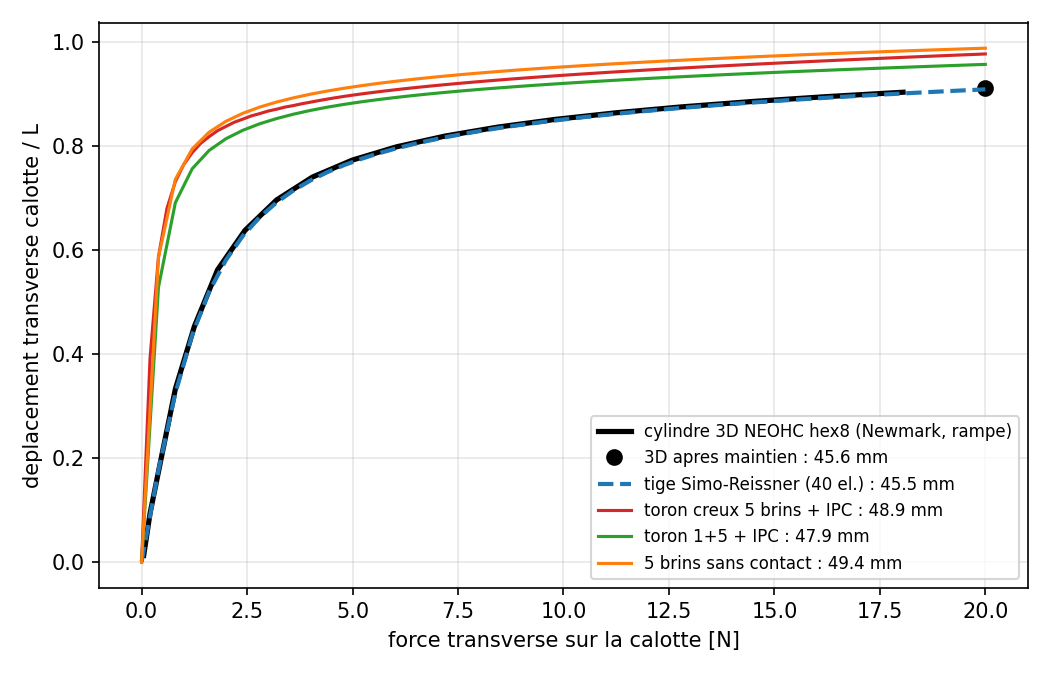
\includegraphics[width=0.78\linewidth]{fig/comparison_force.png}
\caption{Déplacement transverse de la calotte en fonction de la force : la tige
SR suit le calcul 3D à 0,3\,\% près ; les torons, dont la rigidité de flexion
glissante vaut environ $0{,}2EI$, sont beaucoup plus souples.}
\end{figure}

\begin{center}
\small
\begin{tabular}{ccccc}
\toprule
$z/L$ & 3D & tige SR & brins (moy. $\pm$ écart) & plan du toron\\
\midrule
0,05 & 17,3$^\circ$ & 19,0$^\circ$ & 34,8 $\pm$ 4,9$^\circ$ & 4,8$^\circ$\\
0,1 & 33,9$^\circ$ & 34,4$^\circ$ & 55,1 $\pm$ 4,8$^\circ$ & 15,5$^\circ$\\
0,2 & 56,9$^\circ$ & 56,3$^\circ$ & 74,6 $\pm$ 5,7$^\circ$ & 37,3$^\circ$\\
0,4 & 78,6$^\circ$ & 77,8$^\circ$ & 84,5 $\pm$ 5,5$^\circ$ & 87,6$^\circ$\\
0,6 & 86,1$^\circ$ & 85,5$^\circ$ & 88,5 $\pm$ 4,8$^\circ$ & 114$^\circ$\\
0,8 & 88,5$^\circ$ & 88,2$^\circ$ & 93,1 $\pm$ 3,9$^\circ$ & 110$^\circ$\\
\bottomrule
\end{tabular}
\end{center}

\begin{figure}[ht]
\centering
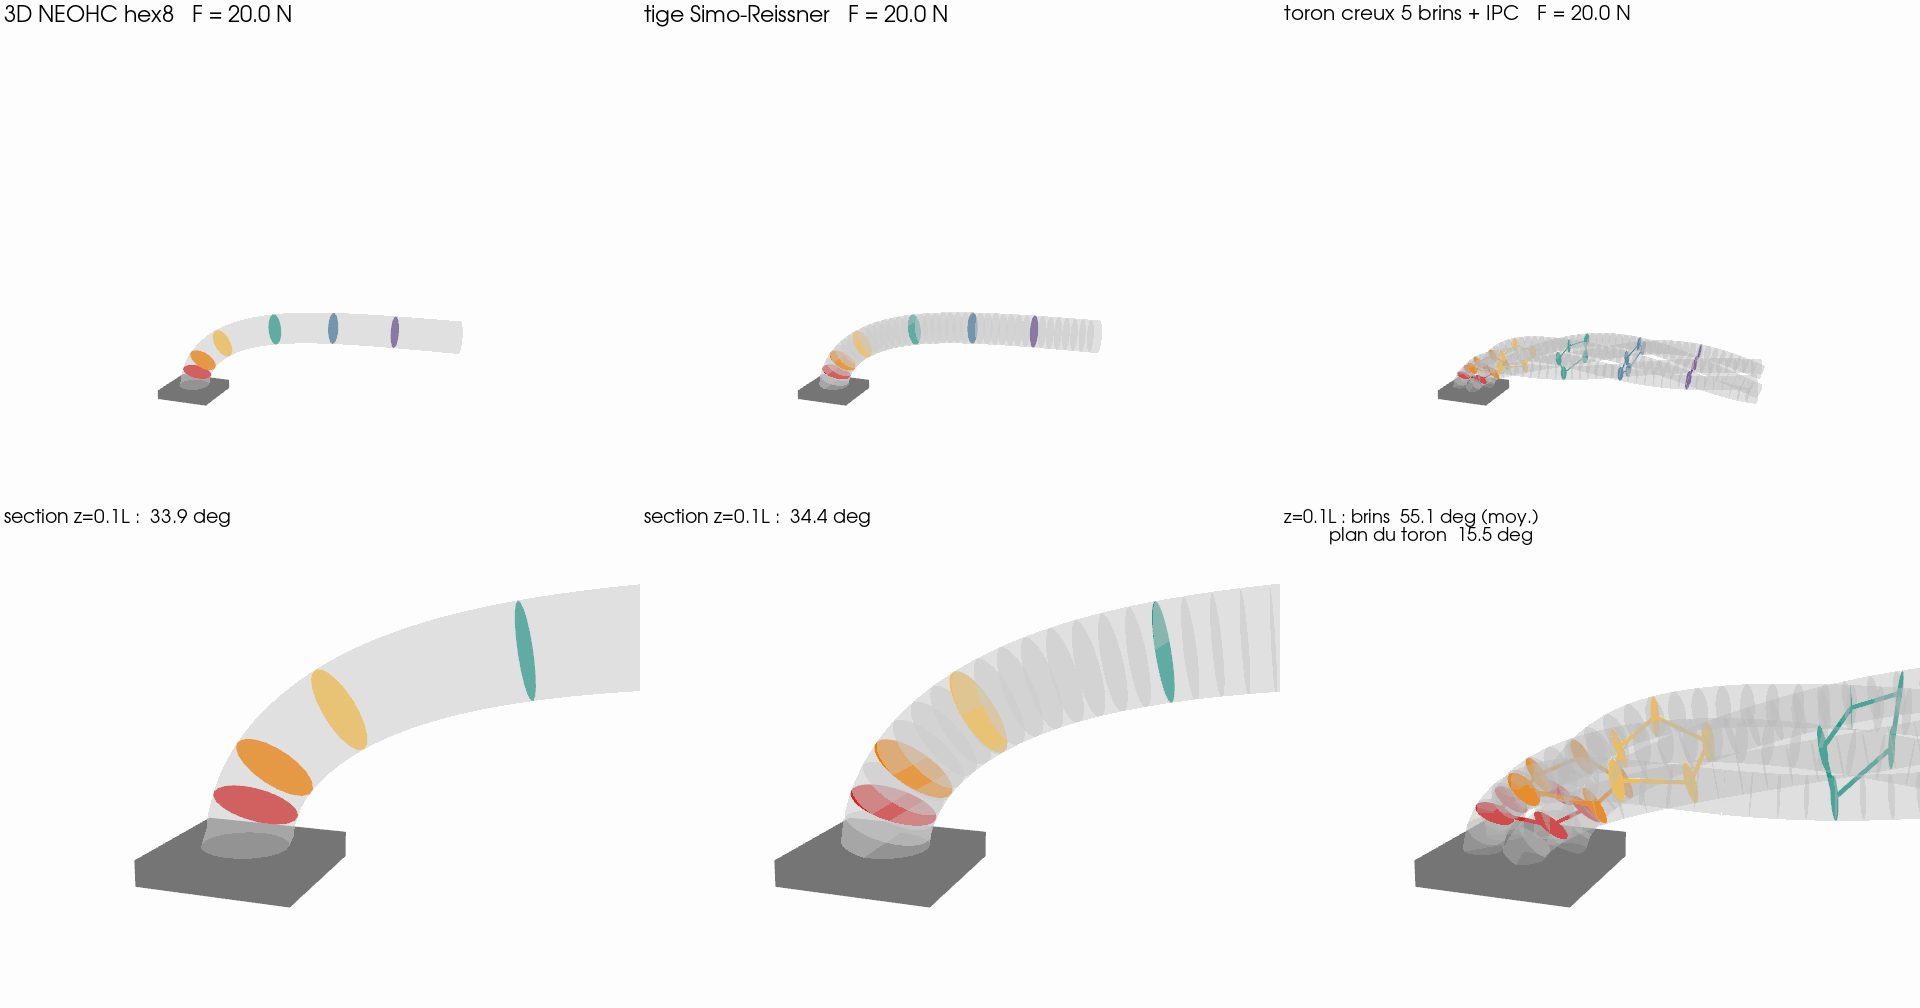
\includegraphics[width=\linewidth]{fig/section_rotation_3d_beam_strand_final.png}
\caption{Rotation des sections à 20~N : cylindre 3D, tige SR et toron creux de
cinq brins avec contact IPC (en bas, zoom sur l'encastrement). La tige reproduit
la rotation de section du 3D, y compris le cisaillement près de l'encastrement ;
dans le toron, les brins glissent axialement et fléchissent chacun autour de
leur axe : la section du toron ne reste pas plane.}
\end{figure}

La tige SR reproduit la rotation de section du 3D à moins de $1^\circ$ sauf au
ras de l'encastrement, et capte le cisaillement de la couche limite (fibre
moyenne entre $0{,}05L$ et $0{,}2L$ à $41{,}9^\circ$ en 3D contre $42{,}2^\circ$).
Dans le toron, chaque brin tourne bien plus que la section pleine ($55^\circ$
contre $34^\circ$ à $0{,}1L$) tandis que le plan ajusté sur les cinq brins tourne
peu : c'est la signature du glissement entre brins, que seul un modèle à brins
avec contact peut représenter.

%======================================================================
\section{Synthèse comparative}
\begin{center}
\small
\begin{tabularx}{\linewidth}{>{\raggedright}p{2.6cm}>{\raggedright}X>{\raggedright}X>{\raggedright\arraybackslash}X}
\toprule
 & Kirchhoff & Corotationnel (fedoo) & SR exact (fedoo)\\
\midrule
Cinématique & ligne $C^1$ + torsion & repère rigide d'élément + Timoshenko linéaire local & $\mathbb R^3\times SO(3)$, $\Gam$, $\Kv$ exacts\\
Cisaillement & aucun & linéaire, local & fini, exact\\
Déformations & rotations finies ; selon la loi & petites déformations locales & arbitraires (limitées par la loi), $|K|L_e<\pi$\\
Symétrie de la tangente & selon la paramétrisation & non symétrique, même à l'équilibre & 2D symétrique ; 3D $\mathbf A-\mathbf A^T=-\mathrm{bd}[\hatv r_\theta]$\\
Coût & moins de ddl, base $C^1$ & le moins cher par élément & même ordre que le corotationnel\\
Objectivité & oui si rotations relatives \cite{meier2014} & oui (repère) & oui (CJ), $10^{-12}$\\
Dépendance au chemin & selon la formulation & angle rigide cumulé en 2D ; 3D \averif & aucune (total), testé\\
Torons + contact & efficace pour fils très élancés \cite{costello1997} ; cisaillement d'encastrement perdu & acceptable en petites déformations & robuste ; hélices exactes ; tangente exacte pour le Newton IPC\\
\bottomrule
\end{tabularx}
\end{center}

%======================================================================
\section{Limites et perspectives}
\begin{itemize}
\item \textbf{Fibres en $\ln\lambda$} (section~\ref{sec:fibres}) et lois
hyperélastiques condensées par simcoon ; filtre de validité $\min\lambda>0$
dans la recherche linéaire.
\item \textbf{Fibres en cisaillement} (\code{nshr=2}) : torsion et cisaillement
issus du matériau plutôt que de $kGA$ et $GJ$ élastiques.
\item \textbf{Dynamique sur $SO(3)$} : inertie rotative et terme gyroscopique,
Newmark en spins \cite{simovuquoc1988}, schémas énergie--moment
\cite{simo1995,romero2002,jelenic1998}, generalized-$\alpha$ sur groupes de Lie
\cite{bruls2010}. Les intégrateurs \code{fd.time} actuels agissent
additivement et ne conviennent pas au bloc \code{Rot} au-delà de petits
incréments.
\item \textbf{Gauchissement et sections déformables}
\cite{simovuquoc1991,gruttmann1998,durville2012}.
\item \textbf{Éléments d'ordre supérieur} : interpolation CJ à $n$ nœuds
\cite{jelenic1999}.
\item \textbf{Points à auditer} : \code{commit\_nodal\_rotations} stocke
$d\mathbf U=\log(\Lam_{\text{new}}\exp(\mathbf U)^T)$, de sorte que
$\exp(\mathbf U+d\mathbf U)\ne\Lam_{\text{new}}$ en général : tout consommateur
lisant les ddl \code{Rot} comme vecteurs rotation totaux est approché aux
grandes rotations ; vérifier l'auto-équilibre de la force corotationnelle ;
mesurer l'identité de symétrie dans fedoo.
\end{itemize}

%======================================================================
\begin{thebibliography}{99}\small
\bibitem{kirchhoff1859} G. Kirchhoff, Über das Gleichgewicht und die Bewegung eines unendlich dünnen elastischen Stabes, \emph{J. reine angew. Math.} 56 (1859) 285--313.
\bibitem{love1927} A.E.H. Love, \emph{A Treatise on the Mathematical Theory of Elasticity}, 4th ed., Cambridge Univ. Press, 1927.
\bibitem{antman2005} S.S. Antman, \emph{Nonlinear Problems of Elasticity}, 2nd ed., Springer, 2005.
\bibitem{reissner1972} E. Reissner, On one-dimensional finite-strain beam theory: the plane problem, \emph{ZAMP} 23 (1972) 795--804.
\bibitem{reissner1981} E. Reissner, On finite deformations of space-curved beams, \emph{ZAMP} 32 (1981) 734--744.
\bibitem{simo1985} J.C. Simo, A finite strain beam formulation. The three-dimensional dynamic problem. Part I, \emph{CMAME} 49 (1985) 55--70.
\bibitem{simovuquoc1986} J.C. Simo, L. Vu-Quoc, A three-dimensional finite-strain rod model. Part II: Computational aspects, \emph{CMAME} 58 (1986) 79--116.
\bibitem{simovuquoc1988} J.C. Simo, L. Vu-Quoc, On the dynamics in space of rods undergoing large motions --- a geometrically exact approach, \emph{CMAME} 66 (1988) 125--161.
\bibitem{simovuquoc1991} J.C. Simo, L. Vu-Quoc, A geometrically-exact rod model incorporating shear and torsion-warping deformation, \emph{IJSS} 27 (1991) 371--393.
\bibitem{simo1992hessian} J.C. Simo, The (symmetric) Hessian for geometrically nonlinear models in solid mechanics, \emph{CMAME} 96 (1992) 189--200.
\bibitem{simo1995} J.C. Simo, N. Tarnow, M. Doblaré, Non-linear dynamics of three-dimensional rods: exact energy and momentum conserving algorithms, \emph{IJNME} 38 (1995) 1431--1473.
\bibitem{argyris1982} J. Argyris, An excursion into large rotations, \emph{CMAME} 32 (1982) 85--155.
\bibitem{cardona1988} A. Cardona, M. Géradin, A beam finite element non-linear theory with finite rotations, \emph{IJNME} 26 (1988) 2403--2438.
\bibitem{ibrahimbegovic1995} A. Ibrahimbegović, F. Frey, I. Kožar, Computational aspects of vector-like parametrization of three-dimensional finite rotations, \emph{IJNME} 38 (1995) 3653--3673.
\bibitem{crisfield1999} M.A. Crisfield, G. Jelenić, Objectivity of strain measures in the geometrically exact three-dimensional beam theory and its finite-element implementation, \emph{Proc. R. Soc. Lond. A} 455 (1999) 1125--1147.
\bibitem{jelenic1999} G. Jelenić, M.A. Crisfield, Geometrically exact 3D beam theory: implementation of a strain-invariant finite element for statics and dynamics, \emph{CMAME} 171 (1999) 141--171.
\bibitem{jelenic1998} G. Jelenić, M.A. Crisfield, Interpolation of rotational variables in nonlinear dynamics of 3D beams, \emph{IJNME} 43 (1998) 1193--1222.
\bibitem{romero2002} I. Romero, F. Armero, An objective finite element approximation of the kinematics of geometrically exact rods and its use in the formulation of an energy-momentum conserving scheme in dynamics, \emph{IJNME} 54 (2002) 1683--1716.
\bibitem{betsch2002} P. Betsch, P. Steinmann, Frame-indifferent beam finite elements based on the geometrically exact beam theory, \emph{IJNME} 54 (2002) 1775--1788.
\bibitem{romero2004} I. Romero, The interpolation of rotations and its application to finite element models of geometrically exact rods, \emph{Comput. Mech.} 34 (2004) 121--133.
\bibitem{makinen2007} J. Mäkinen, Total Lagrangian Reissner's geometrically exact beam element without singularities, \emph{IJNME} 70 (2007) 1009--1048.
\bibitem{meier2014} C. Meier, A. Popp, W.A. Wall, An objective 3D large deformation finite element formulation for geometrically exact curved Kirchhoff rods, \emph{CMAME} 278 (2014) 445--478.
\bibitem{meier2019} C. Meier, A. Popp, W.A. Wall, Geometrically exact finite element formulations for slender beams: Kirchhoff--Love theory versus Simo--Reissner theory, \emph{Arch. Comput. Methods Eng.} 26 (2019) 163--243.
\bibitem{belytschko1973} T. Belytschko, B.J. Hsieh, Non-linear transient finite element analysis with convected co-ordinates, \emph{IJNME} 7 (1973) 255--271.
\bibitem{rankin1986} C.C. Rankin, F.A. Brogan, An element independent corotational procedure for the treatment of large rotations, \emph{J. Press. Vessel Technol.} 108 (1986) 165--174.
\bibitem{crisfield1990} M.A. Crisfield, A consistent co-rotational formulation for non-linear, three-dimensional, beam-elements, \emph{CMAME} 81 (1990) 131--150.
\bibitem{nouromid1991} B. Nour-Omid, C.C. Rankin, Finite rotation analysis and consistent linearization using projectors, \emph{CMAME} 93 (1991) 353--384.
\bibitem{crisfield1997} M.A. Crisfield, \emph{Non-linear Finite Element Analysis of Solids and Structures, Vol. 2: Advanced Topics}, Wiley, 1997.
\bibitem{battini2002} J.-M. Battini, C. Pacoste, Co-rotational beam elements with warping effects in instability problems, \emph{CMAME} 191 (2002) 1755--1789.
\bibitem{felippa2005} C.A. Felippa, B. Haugen, A unified formulation of small-strain corotational finite elements: I. Theory, \emph{CMAME} 194 (2005) 2285--2335.
\bibitem{gruttmann1998} F. Gruttmann, R. Sauer, W. Wagner, A geometrical nonlinear eccentric 3D-beam element with arbitrary cross-sections, \emph{CMAME} 160 (1998) 383--400.
\bibitem{durville2012} D. Durville, Contact-friction modeling within elastic beam assemblies: an application to knot tightening, \emph{Comput. Mech.} 49 (2012) 687--707.
\bibitem{costello1997} G.A. Costello, \emph{Theory of Wire Rope}, 2nd ed., Springer, 1997.
\bibitem{hoger1987} A. Hoger, The stress conjugate to logarithmic strain, \emph{IJSS} 23 (1987) 1645--1656.
\bibitem{xiao1997} H. Xiao, O.T. Bruhns, A. Meyers, Logarithmic strain, logarithmic spin and logarithmic rate, \emph{Acta Mech.} 124 (1997) 89--105.
\bibitem{xiao1999} H. Xiao, O.T. Bruhns, A. Meyers, Existence and uniqueness of the integrable-exactly hypoelastic equation and its significance to finite inelasticity, \emph{Acta Mech.} 138 (1999) 31--50.
\bibitem{anand1979} L. Anand, On H. Hencky's approximate strain-energy function for moderate deformations, \emph{J. Appl. Mech.} 46 (1979) 78--82.
\bibitem{bruhns2001} O.T. Bruhns, H. Xiao, A. Meyers, Constitutive inequalities for an isotropic elastic strain-energy function based on Hencky's logarithmic strain tensor, \emph{Proc. R. Soc. Lond. A} 457 (2001) 2207--2226.
\bibitem{eterovic1990} A.L. Eterovic, K.-J. Bathe, A hyperelastic-based large strain elasto-plastic constitutive formulation with combined isotropic-kinematic hardening using the logarithmic stress and strain measures, \emph{IJNME} 30 (1990) 1099--1114.
\bibitem{miehe2002} C. Miehe, N. Apel, M. Lambrecht, Anisotropic additive plasticity in the logarithmic strain space, \emph{CMAME} 191 (2002) 5383--5425.
\bibitem{dienes1979} J.K. Dienes, On the analysis of rotation and stress rate in deforming bodies, \emph{Acta Mech.} 32 (1979) 217--232.
\bibitem{bruls2010} O. Brüls, A. Cardona, On the use of Lie group time integrators in multibody dynamics, \emph{J. Comput. Nonlinear Dyn.} 5 (2010) 031002.
\end{thebibliography}

\end{document}
